\documentclass[12pt,subf,href,colorlinks=true]{article}



\usepackage[a4paper,nohead,includefoot,mag=1000,
            margin=2cm,footskip=1cm]{geometry}
%\usepackage[T2A]{fontenc}
%\usepackage[cp1251]{inputenc}
%\usepackage{pscyr}
%\renewcommand{\rmdefault}{ftm}
\usepackage{cmap}
\usepackage[utf8]{inputenc}
%\usepackage[TS1,T2A]{fontenc}
\usepackage[russian]{babel}
\usepackage{tabularx}
\usepackage{hyperref}
\ifpdf\usepackage{epstopdf}\fi
\hypersetup{
    colorlinks=true,
    linkcolor=blue,
    filecolor=magenta,      
    urlcolor=blue,
}
\usepackage{listings}
\usepackage{algorithm}
\usepackage{algpseudocode}

\title{Задание №3: Программная реализация графического конвейера и графического API}
\author{Владимир Фролов}
\date{\today}

\usepackage{graphicx}
\graphicspath{{img/}}
\renewcommand{\baselinestretch}{1.25}

% listings

\usepackage{color} 
\usepackage{listings} 
\usepackage{caption}
\DeclareCaptionFont{white}{\color{white}} 
\DeclareCaptionFormat{listing}{\colorbox{gray}{\parbox{\textwidth}{#1#2#3}}}
\captionsetup[lstlisting]{format=listing,labelfont=white,textfont=white}


\lstset{ %
language=C,                
stepnumber=1,              
tabsize=2,                 
}

\begin{document}
\maketitle

\begin{abstract}
	
\noindent Цель задания: закрепить на практике основные работы графического конвейера через его реализацию.

\begin{itemize}

\item Закрепление знаний о трёхмерных преобразованиях и базовых математических операциях.
\item Изучение базовых принципов работы графического конвейера;
\item (Дополнительно) Программируемая функциональность граф-конвейера.
\item (Дополнительно) Карты теней	 
	 
\end{itemize}	

\end{abstract}


\begin{figure}
	\begin{center}
		\begin{tabular}{c c}
			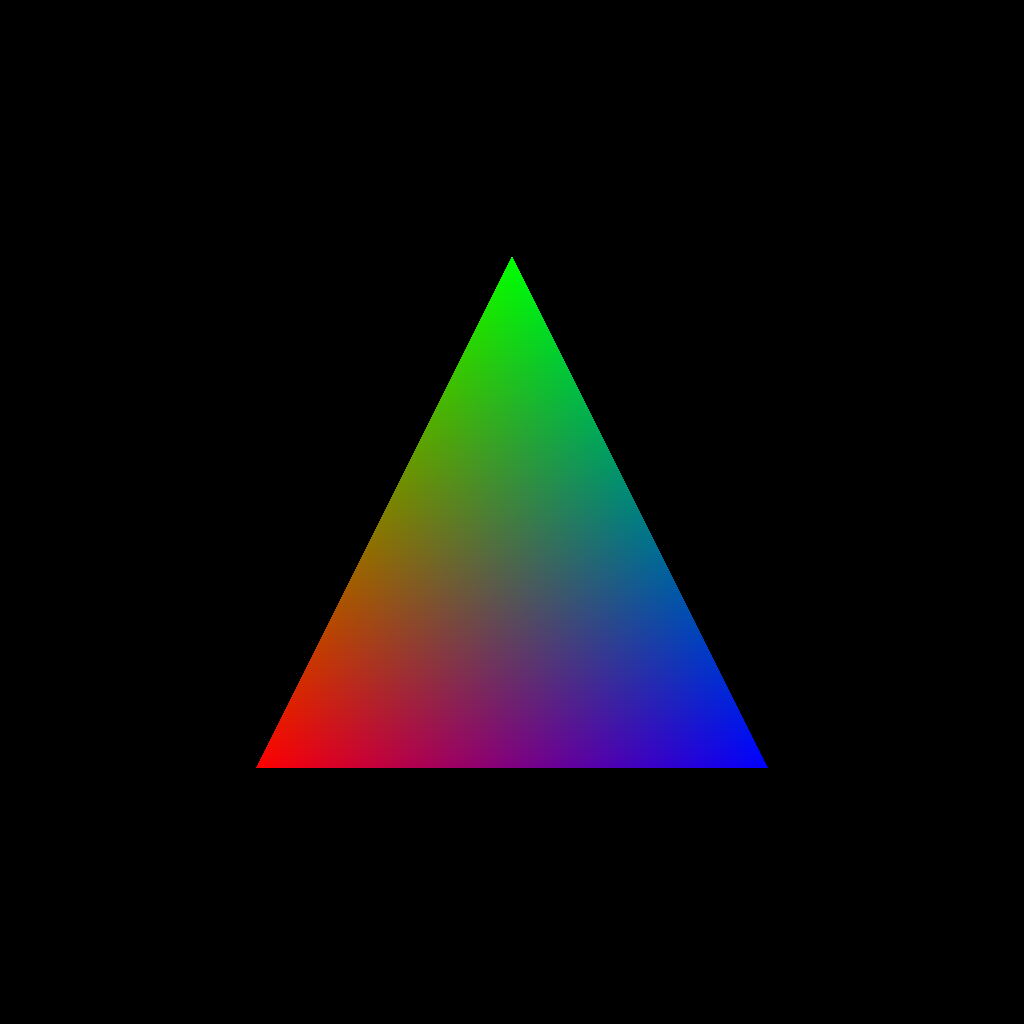
\includegraphics[width=0.25\textwidth]{img/wref_01.png} & 
			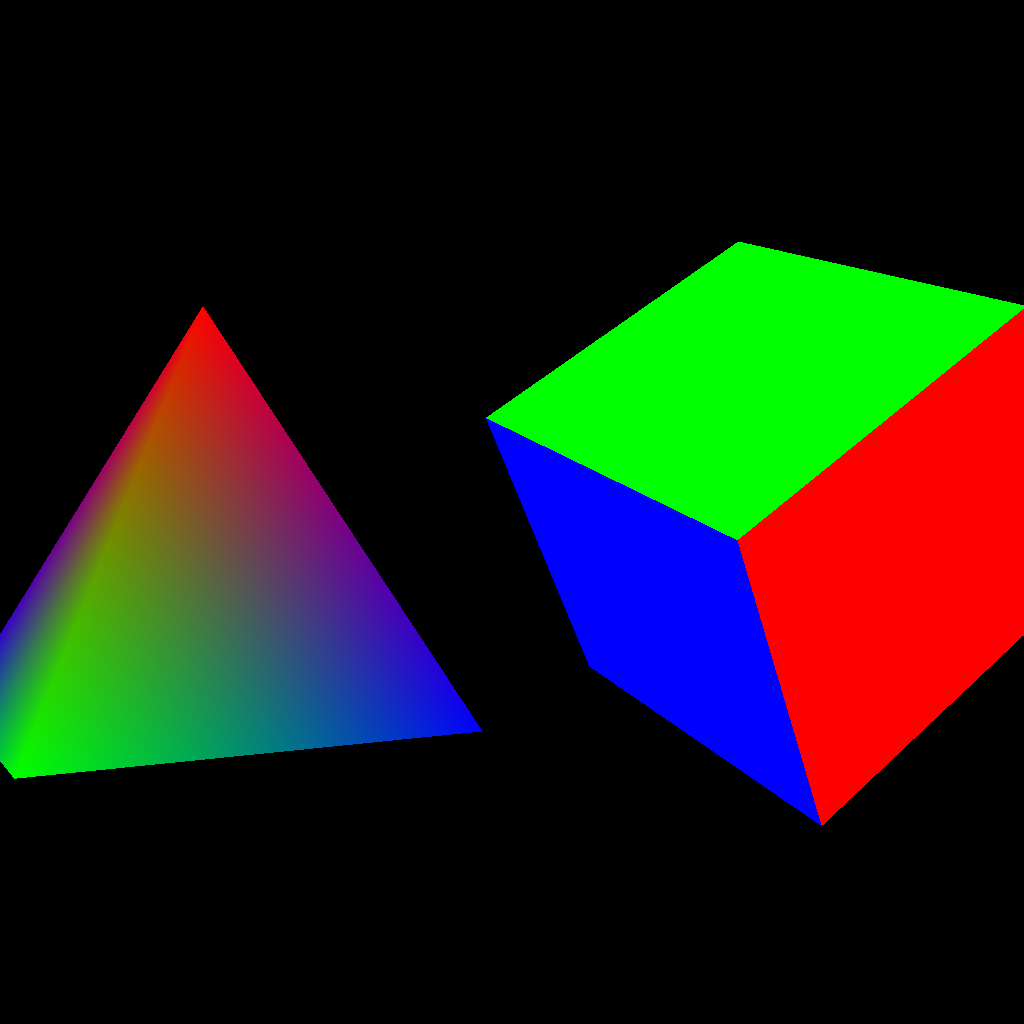
\includegraphics[width=0.25\textwidth]{img/wref_03.png} \\ 
			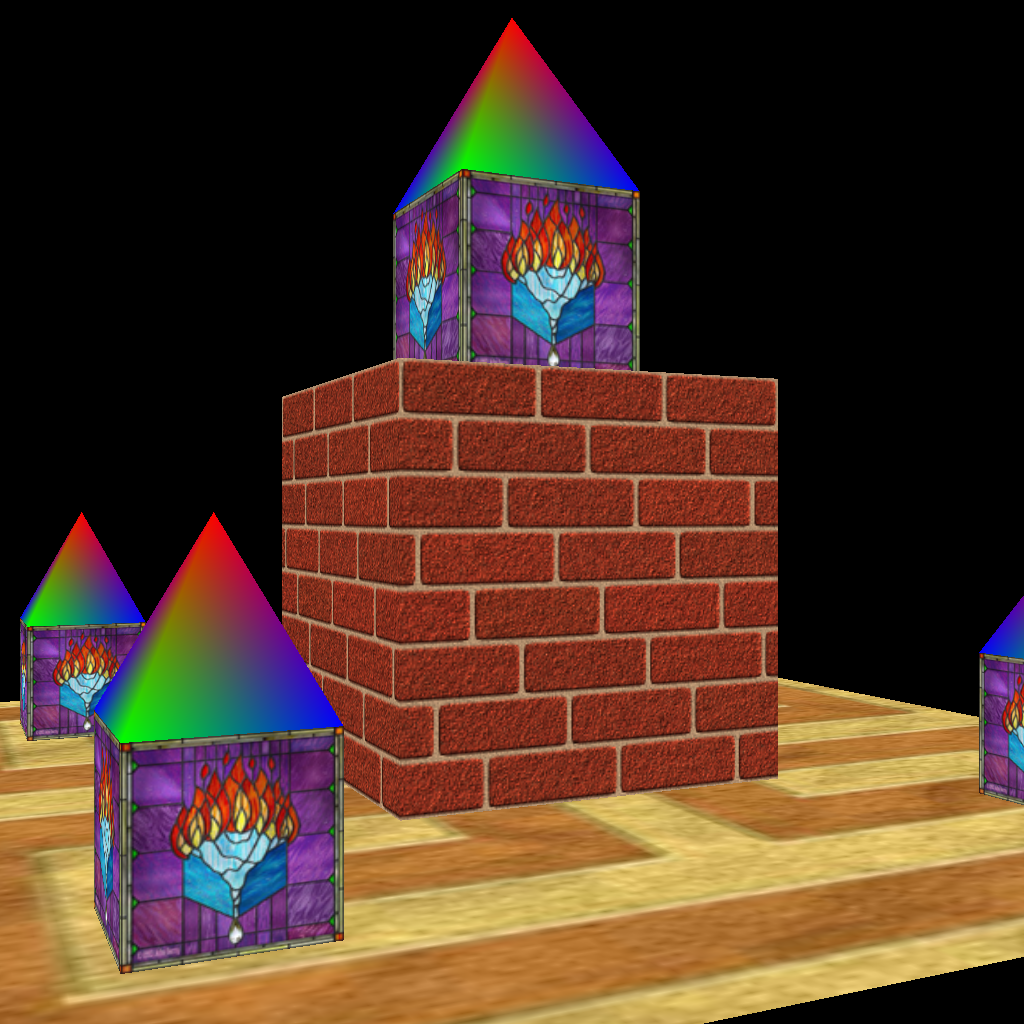
\includegraphics[width=0.25\textwidth]{img/wref_05.png} &
			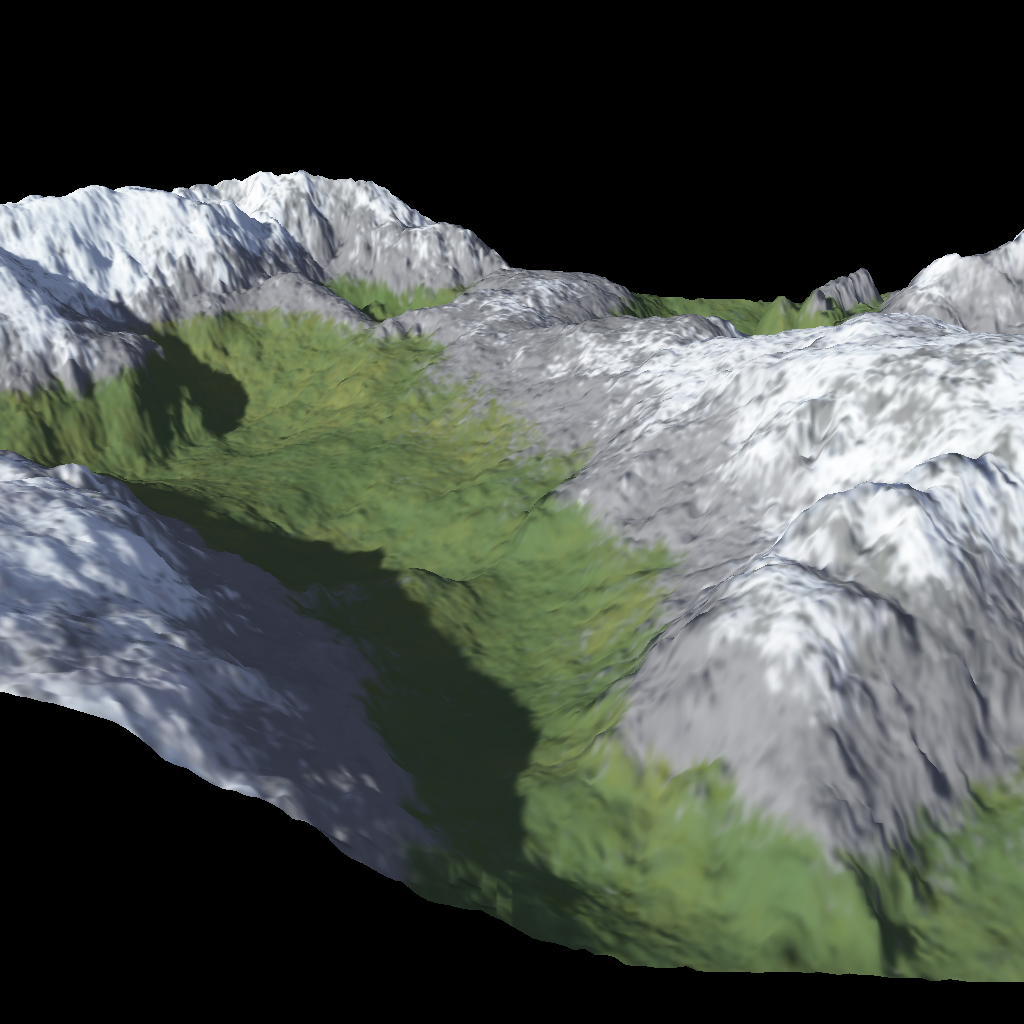
\includegraphics[width=0.25\textwidth]{img/wref_08.png} \\
		\end{tabular}
		\caption{Изображения некоторых тестовых сцен}
		\label{fig:images}
	\end{center}
\end{figure}

\section{Базовая часть: 10 баллов }

Необходимо реализовать базовый алгоритм растеризации 3D моделей с поддержкой текстурирования.

\begin{itemize}
  \item Необходимо реализовать заливку треугольника константным цветом (1 балл).
  \item Необходимо реализовать интерполяцию цвета (2 балла).
  \item Необходимо реализовать интерполяцию текстурных координат с перспективной коррекцией (3 балла).
  \item Необходимо реализовать алгоритм буфера глубины для корректного отображения ближних и дальних объектов (4 балла).
  \item Для каждого изображения необходимо вывести время его рендеринга. При невыполнении этого требования баллы за базовую часть будут снижены вдвое!
  \item К заданию прилагается эталонная реализация через OpenGL 1.0. Для успешного выполнения задания необходимо получить хотя бы похожие (а в идеале совпадающие) с эталонными изображения на всех 8 тестах (рис. \ref{fig:images}). При невыполнении этого требования баллы за базовую часть будут снижены на усмотрение проверяющего.
\end{itemize}

\section{Дополнительная часть: 15 баллов макс.}

\begin{itemize}
	
	\item Синтез последовательности изображений, содержаших поворот сцены вокруг центра координат или вращение некоторой 3D модели вокруг её центра (+1 балл). 
  
    \begin{itemize}
    \item Используйте ffmpeg чтобы получить видео-последовательность из набора изображений:
    \begin{verbatim}ffmpeg -framerate 25 -pattern\_type glob -i '*.bmp' out.gif \end{verbatim}
    
    \item В качестве альтернативного решения Вы можете выводить изображений в окно (проверка вашего задания будет осущесвлятьтся на Linux с оконной системой X11, как в примере для эталонной реализации). В этом случае пожалуйста выведите частоту кадров в название окна или в командную строку.
    \end{itemize}
    
	\item Загрузка и рендеринг ``.obj'' файлов (3 балла).
    \begin{itemize}
    	\item Необходимо реализовать визуализацию как минимум 2 разных моделей
    	\item Вы можете использовать и другой входной формат 3D моделей.
    \end{itemize}		
		
	\item Реализия фрагментных шейдеров через указатели на функции (или аналогичную функциональность вашего языка программирования) (3 балла).
	
	\begin{itemize}
	  \item Добавьте необходимую входную информацию в структуру PipelineStateObject;	
	  \item Необходимо реализовать рассчёт освещения во фрагментном шейдере (без этого пункт не засчитывается).
	\end{itemize}

    \item Необходимо реализовать блочный алгоритм растеризации (2 балла).
    
    \item Необходимо применить векторизацию кода для блочного растеризатора и фрагментных шейдеров при помощи Intel ISPC (2 балла).
    
    \begin{itemize}
      \item В этом пункте необходимо реализовать рассчёт освещения во фрагментном шейдере (без этого пункт не засчитывается).
      \item Все векторизованные шейдеры должны быть собраны в объектные файлы и статически прилинкованы к проекты.
      \item Необходимо привести сравнение времени выполнения для обычных и векторизованных шейдеров.
    \end{itemize}
	
	\item Необходимо реализовать алгоритм карт теней. Необходимо продемонстрировать самозатенение или отбрасывание теней с одного 3D объекта на другие (4 балла).
	
	\item Растеризация квад-мешей  (+3 балла).
	\begin{itemize}
	  \item В последнее время стали популярны меши, состоящие из четырё-угольников \cite{quadmeshes_about}. Преобразование таких мешей в треугольные снижает эффективность блочных алгоритмов растеризации на границе двух треугнольников, образующих квад. Необходимо реализовать алгоритм растеризации квадов и сравнить время работы с растеризацией треугольников.
	  
	  \item Существенно-непланарные квады необходимо всё-равно разбивать на треугольники.
	  
	  \item Данный пункт имеет смысл выполнять только если Вы реализуете блочный векторизованный алгоритм. 
	  
	  \item Подготовленные для задания квад-меши можно найти здесь: \cite{quadmeshes}. 
	   
	\end{itemize}
	
\end{itemize}

\section{Порядок выполнения задания}

\begin{enumerate}
\item Скачайте или склонируйте себе шаблон для выполнения задания \cite{ourtemplate}
  \begin{itemize}
	\item Пожалуйста не выкладывайте Ваше \textbf{решение} в открытый доступ. Дайте возможность другим людям достичь результата самостоятельно.
  \end{itemize}

\item Соберите шаблон с эталонной реализацией и сгенерируйте эталонные изображения
  \begin{itemize}
  \item \begin{verbatim} mkdir build && cd build \end{verbatim}
  \item \begin{verbatim} cmake -DCMAKE_BUILD_TYPE=Release (или Debug) -DUSE_OPENGL=ON .. \end{verbatim}
  \item \begin{verbatim} make -j 8 \end{verbatim}
  \item Запустите полученную програму
  \end{itemize}

\item Отключите эталонную реализацию и приступайте к выполнению задания
   \begin{itemize}
  	\item \begin{verbatim} cmake -DCMAKE_BUILD_TYPE=Release (или Debug) -DUSE_OPENGL=OFF .. \end{verbatim}
  	\item \begin{verbatim} make -j 8 \end{verbatim}
  \end{itemize}

\item Эталонная реализация создаёт окно при помощи X11, поэтому если в Вашей системе это невозможно, попросите товарища сгенерировать эталонные изображения для Вас.

\item Если Вы хотите выполнить задание на другом языке программирования, это допускается при условии совпадения вашей реализации с эталонными изображениями. 

\item Изучите раздел \ref{materials} (Материалы для выполнения задания) и сайт \cite{scratchpixel}.

\end{enumerate}

\section{Порядок сдачи}
Ваша программа должна запускаться без аргументов, производить рендеринг изображений и сохранить их на выходе в bmp формат. Если Вы создаёте окно, то примите во внимание что проверка будет производитьcя на машинах Linux и оконной системой X11 (XWindow).
 
\noindent\textbf{Использование библиотек}: 

Все используемые библиотеки должны быть либо собраны в статические библиотеки для архитектуры x64 c поддержкой AVX2 (-mavx2) под gcc, либо должны поставляться с проектом в виде исходных кодов, и фактически быть его частью. 

PS: строго говоря, для выполнения данного задания Вам не нужны библиотеки. Рекомендуется выполнять задание без них. 

\section{Именование архива}

Архив, который вы загружаете на сайт должен называться по следующему шаблону: \newline <номер\_группы>\_<фамилия>.zip. Фамилию следует писать латинскими символами.

\section{Материалы для выполнения задания}\label{materials}

Итак, Вам неповезло выбрать компьютерную графику в качестве профессии, так что будьте готовы к страданиям. Кроме того Вам выдали это скучнейшее в мире задание c растеризацией треугольников, в котором зачем-то требуется совпадение Вашей реализации с эталонной, написанной на умершем уже 10 лет как OpenGL 1.0.

Что-ж, на практике Вам действительно придётся использовать другие API, шейдеры, GPU и многое другое. Поэтому совершенно точно можно сказать, что выполнив это задание Вы не получите практических навыков. Зато Вы получите громадный буст к их освоению, поскольку будете понимать как графические API, граф. конвейер (и даже современные GPU) устроены внутри. Ведь в действительности там всё не так сложно, как кажется на первый взгляд.

\subsection{Вопрос дизайна графического API}

Вам предлагается реализовать учебный API, в котором функциональность урезана до минимума. Если он Вам не нравится, Вы можете придумать свой API и реализовать предложенный через него.

\subsection{Стадии графического конвейера}

\begin{figure}[h]
	\centering{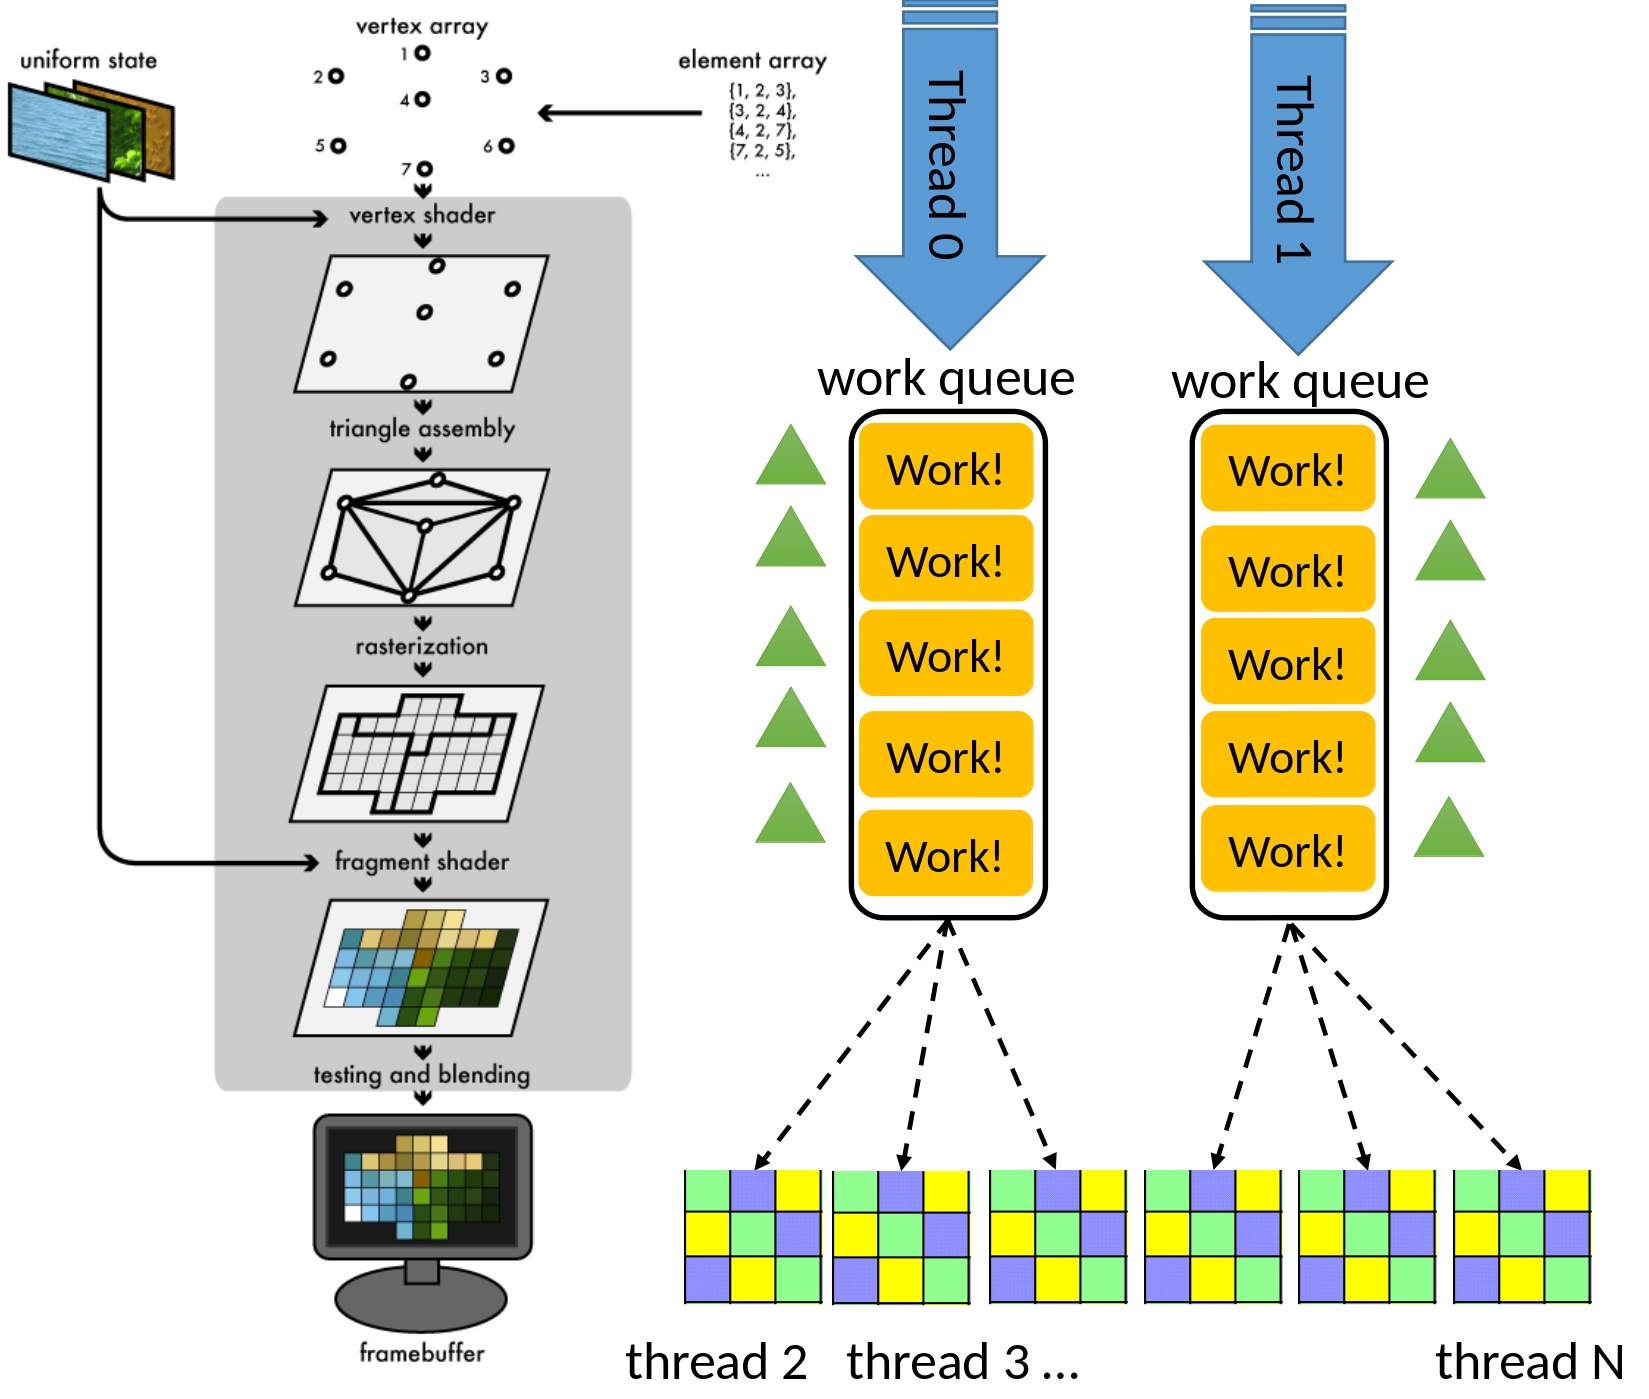
\includegraphics[width=0.5\linewidth]{img/graphicspipeline}}
	\caption{Графический конвейер устроен по схеме производитель-потребитель, где каждая стадия принимает на вход порцию данных, обрабатывает её и передаёт ниже по конвейеру. Как привило, обработка фрагментов гораздо тяжелее геометрических стадий.}
	\label{fig:prodcons}
\end{figure}
%\FloatBarrier

\subsection{Алгоритм растеризации на основе полу-пространства}

\begin{figure}[htb]
	\centering{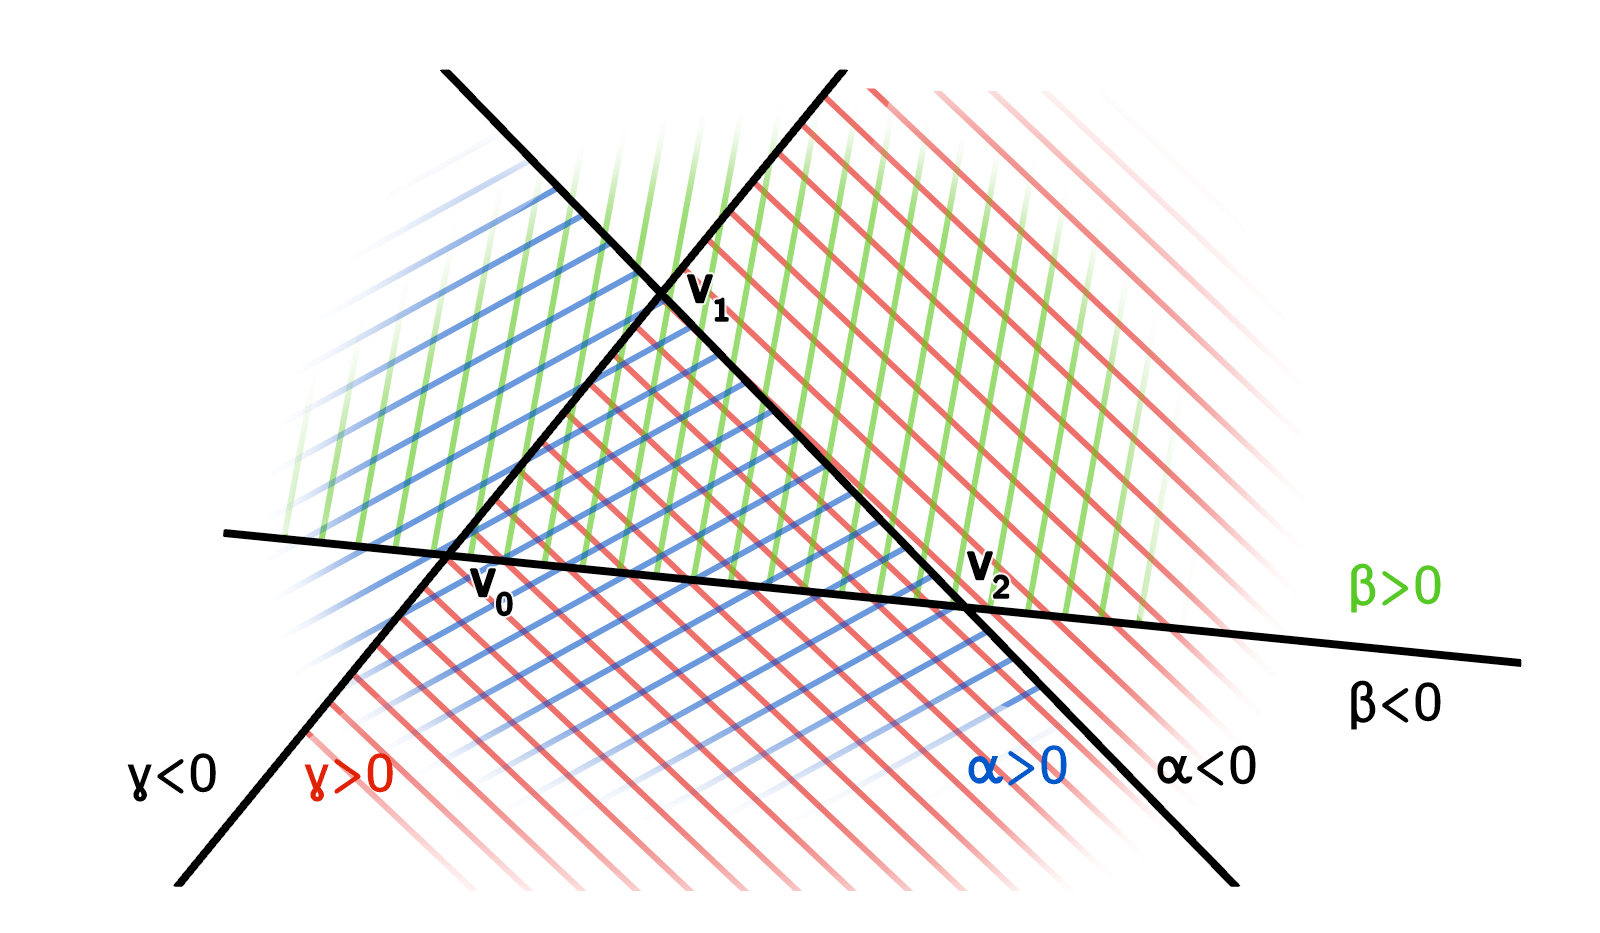
\includegraphics[width=0.5\linewidth]{img/barycentric}}
	\caption{Half-space algorithm idea}
	\label{fig:halfspace}
\end{figure}

\begin{figure}[htb]
	\centering{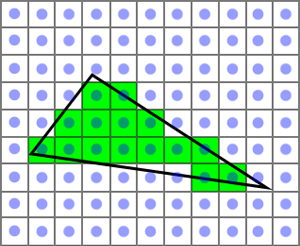
\includegraphics[width=0.25\linewidth]{img/coveragetest}}
	\caption{Standard agreement about covered pixels.  A pixel is considered as overlapped by two-dimensional triangle if its center lies inside the triangle.}
	\label{fig:coveragetest}
\end{figure}

\begin{equation}\label{eq:edgefunction}
	E(A,B,P) = (P.x - A.x) (B.y - A.y) - (P.y - A.y)(B.x - A.x)
\end{equation}

\begin{eqnarray}\label{eq:edgefunction1}
	E_{\alpha}(x,y) = E(A,B,P) &=& (x - A.x)(B.y - A.y) - (y - A.y)(B.x - A.x); \\ \label{eq:edgefunction2}
	E_{\beta} (x,y) = E(B,C,P) &=& (x - B.x)(C.y - B.y) - (y - B.y)(C.x - B.x); \\ \label{eq:edgefunction3}
	E_{\gamma}(x,y) = E(C,A,P) &=& (x - C.x)(A.y - C.y) - (y - C.y)(A.x - C.x).    \label{eq:edgefunction4}
\end{eqnarray}

The most useful property of the \textit{edge-function} is that it can be \textbf{evaluated incrementally} when rasterizer moves along pixels (figure \ref{alg:halfspace}) \cite{Pineda:1988:PAP:378456.378457}. Besides, baricentric coordinates ($u,v,w$) also can be evaluated directly from \textit{edge-function} by multiplying its value with inverse triangle double area which is also evaluated with the \textit{edge-function} (equations \ref{eq:bar1}--\ref{eq:bar4}).

\begin{eqnarray}\label{eq:bar1}
	u(P)        &=& \frac{E(A,B,P)}{E(A,B,C)} ;\\ \label{eq:bar2}
	v(P)        &=& \frac{E(B,C,P)}{E(A,B,C)} ;\\ \label{eq:bar3}
	w(P) = 1-u(P)-v(P) &=& \frac{E(C,A,P)}{E(A,B,C)}. \label{eq:bar4}
\end{eqnarray}

\begin{figure}[h]
	\begin{algorithmic}[1]
		
		\For{y \textbf{in} range minY .. maxY}
		\State Cx1 := Cy1; 
		\State Cx2 := Cy2; 
		\State Cx3 := Cy3; 
		
		\For{x \textbf{in} range minX .. maxX}
		
		\If {$Cx1 > 0\hspace{5pt}\textbf{and}\hspace{5pt}Cx2 > 0\hspace{5pt}\textbf{and}\hspace{5pt}Cx3 > 0$}
		\State u = Cx1*TriAreaInv;
		\State v = Cx2*TriAreaInv;
		\State framebuffer[x,y] := DrawPixel(u, v, 1-u-v);
		\EndIf;
		
		\State Cx1 := Cx1 - Dy12;
		\State Cx2 := Cx2 - Dy23;
		\State Cx3 := Cx3 - Dy31;
		
		\EndFor;
		\State Cy1 := Cy1 + Dx12;
		\State Cy2 := Cy2 + Dx23;
		\State Cy3 := Cy3 + Dx31; 	
		\EndFor;
		
	\end{algorithmic}
	\caption{Half-space rasterization kernel. $Cx*$ and $Cy*$ variables store edge-functions for line and colum respectively. $TriAreaInv=1/E(A,B,C)$ is a constant inverse triangle double area. A triplet of $(u,v, 1-u-v)$ represents baricentric coordinates of a pixel center. }\label{alg:halfspace}
\end{figure}

\begin{thebibliography}{9} 
	
\bibitem{ourtemplate} Шаблон для выполнения задания: https://github.com/FROL256/sw\_gapi\_task 

\bibitem{quadmeshes_about} Bommes, David and Lévy, Bruno and Pietroni, Nico and Puppo, Enrico and Silva, Claudio and Tarini, Marco and Zorin, Denis. Quad‐Mesh Generation and Processing: A Survey. Computer Graphics Forum (2013). 32. 10.1111/cgf.12014. 

\bibitem{quadmeshes} Подготовленные для задания меши из квадов. \newline URL = https://disk.yandex.ru/d/fX-95hx7Z8nDJA 

\bibitem{scratchpixel} Rasterization: a Practical Implementation, Scratchapixel 3.0. A free educational site that progressively introduces you to the world of computer graphics. https://www.scratchapixel.com/lessons/3d-basic-rendering/rasterization-practical-implementation/overview-rasterization-algorithm.html

\end{thebibliography} 

\end{document}
